\documentclass[12pt]{article}
\usepackage{graphicx}
\usepackage{setspace}
\doublespacing

\begin{document}
\begin{titlepage}
    \begin{center}
        \vspace*{1cm}
        \textbf{Vindicating Morey: The 3-Point Attempt Rate and Pace as Predictors of Wins in the NBA
}
        
        \vspace{0.5cm}
        Advanced Statistics
        
        \vspace{1.5cm}
        
        \textbf{Robert "Davis" DeRodes and Lewis Pipkin}\\
        \textbf{May 2nd, 2017}\\
        
        \vfill
                
    \end{center}
\end{titlepage}
\section{Introduction}
	\indent Over the years, basketball has become incredibly popular and engrained in popular culture, American and otherwise. Its popularity is seemingly at its peak right now, especially in the United States and China, and the NBA is the sport's leading league in the world. Athletes all over the world dream of playing in the United States for one of our thirty teams, and this year, the league had players from 41 different countries, including Italy, Croatia, Austria, and South Sudan.\par
As the league grows and changes, the playing style adapts to incorporate new ideas and play styles. Partner this with the growing analytics movement in all major sports (spurred by Billy Beane, general manager of the Oakland Athletics baseball team in the late 1990s), and we see strategies changing on and off the court. Instead of teams taking the players they have and molding a play style to accentuate their strengths, several teams are now looking for certain archetypes of players to fit their preferences or better complement their superstar player(s), if they are lucky enough to have one. \par 
Take the Toronto Raptors: by modern standards, their play style is as old as their mascot. For the past 6 years, the Raptors have been bottom 10 in the league in number of possessions per game. They slowly chip away at their opponents, and their strategy is typically to give the ball to their star, DeMar DeRozan, and let him wind down the shot clock and end possessions with a midrange jumper. We can clearly see this in the Raptors shot chart.\par

\begin{figure}[h]
\centering
\caption{Toronto Raptors 2016-2017 Shot Chart}
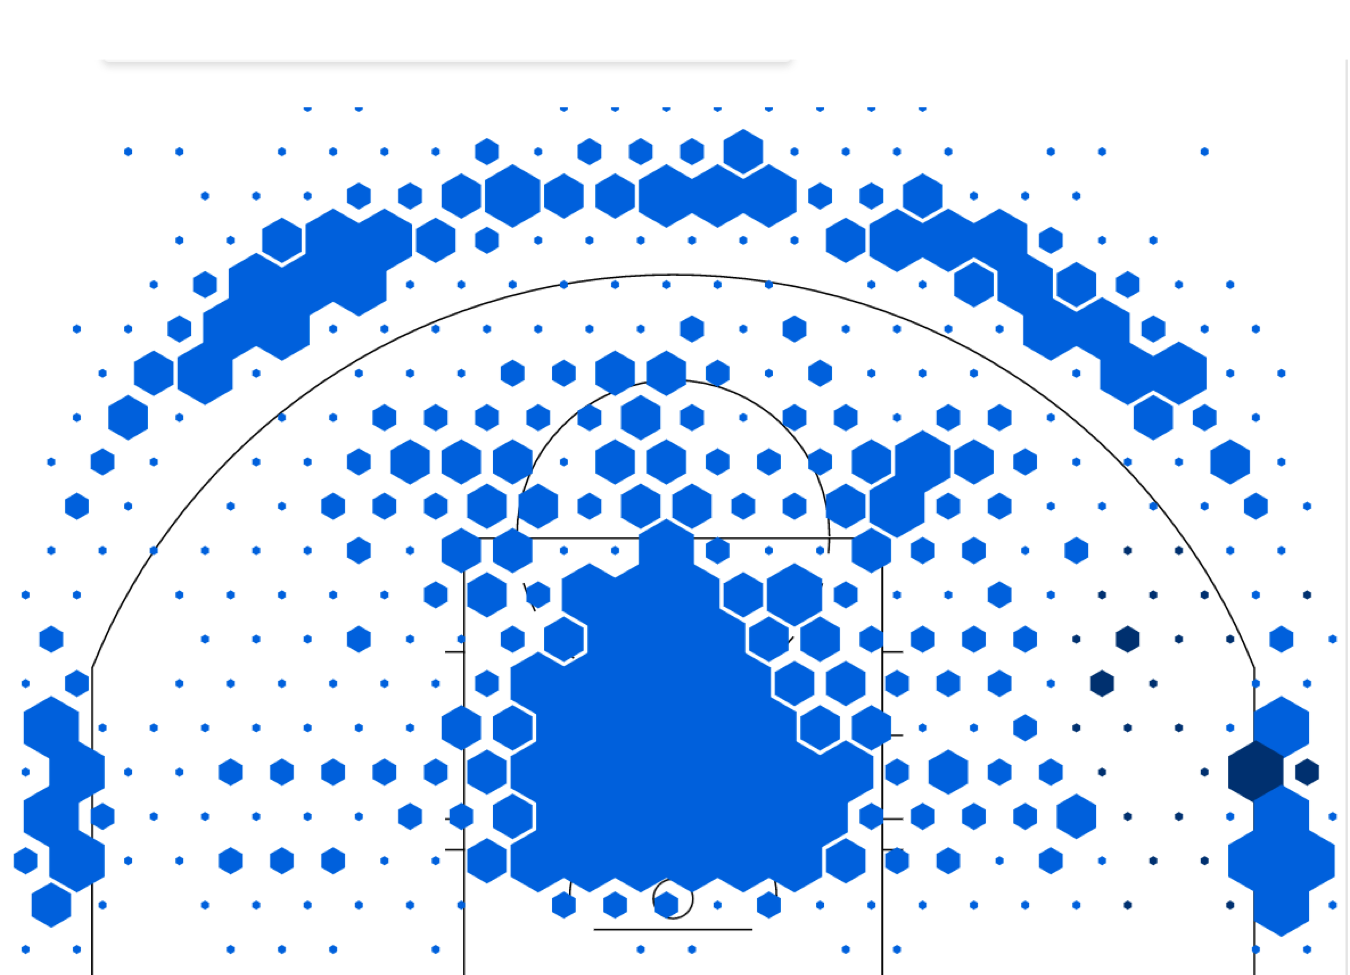
\includegraphics[width=0.5\textwidth]{Raptors}
\end{figure}

        	Then, there are the Houston Rockets. The Rockets have made a revolutionary change in strategy this year: shoot 3-pointers, dunks, and layups, and that's it. Midrange shots are an aberration and should be avoided due to their relative inefficiency. Layups and dunks are highly efficient shots, as they are very hard to miss; in 2017, the league average shooting percentage on dunks and layups was 63.1$\%$, meaning that for every dunk or layup attempt, teams gained an average of 1.26 points. The league average on midrange jumpers, on the other hand, was 41.2$\%$, meaning teams gained only .82 points per shot. Clearly, dunks and layups are the better, more efficient option. The average 3-point shooting percentage across the league was 35.8$\%$, so teams gained about 1.07 points per 3-point shot. They're harder to make, but each individual shot gives teams more points in expectation which explains why some teams have been letting the 3-pointers fly at increasingly higher rates in the name of efficiency. One can see the jarring comparison between the traditional Raptors' and the analytical Rockets' shot charts (see figure 2) as the Rockets have almost no midrange shots in their shot chart and a plethora of 3-pointers and points in the paint.\par
\begin{figure}[h]
\centering
\caption{Houston Rockets 2016-2017 Shot Chart}
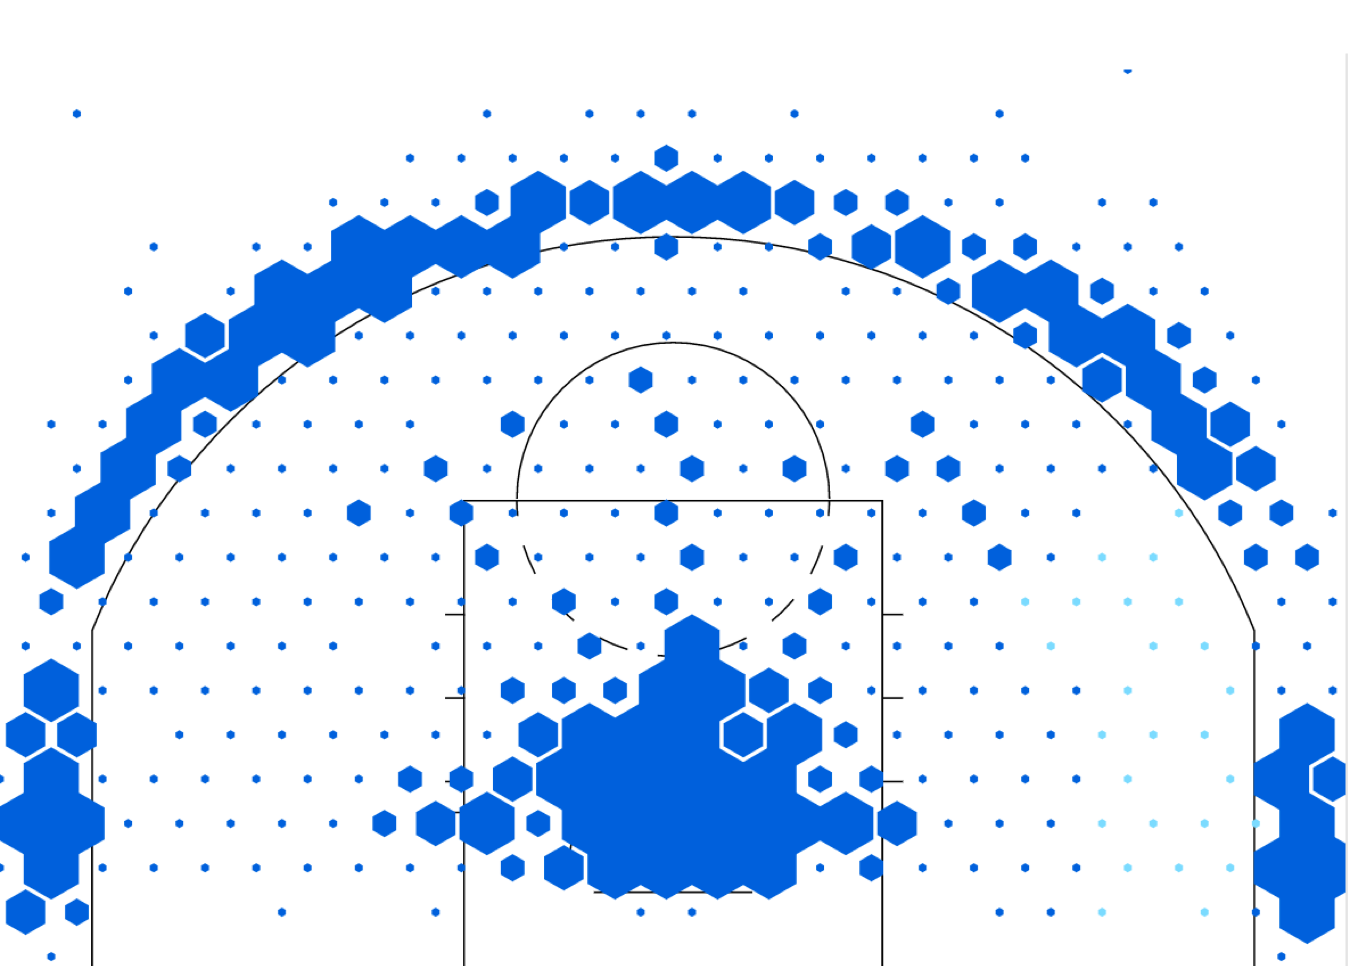
\includegraphics[width=0.5\textwidth]{Rockets}
\end{figure}
        	With the knowledge of the added efficiency given from 3-pointers and points in the paint, the Houston Rockets completely retooled their roster from the year before, giving their starting point guard James Harden the reigns to drive for layups and pass the ball out to one of the four high-percentage shooters outside of the arc if his path is too congested. This system, built under GM Daryl Morey---a statistician, graduate of Northwestern and MIT, and co-founder of the MIT Sloan Sports Analytics Conference---has become wildly successful, as the Rockets shot up to third place in the NBA this year. Several teams, including the seemingly invincible Golden State Warriors, have now adopted this play style, making Morey Ball $the$ NBA revolution in the 21st century. \par
Morey's philosophy of the game has unquestionably ushered in a new era of basketball quantified mostly by a higher attempt rate of 3 pointers and an increased pace --- a metric that takes into account the total amount of possessions in a basketball game. In model 1, we can clearly see that since Morey has entered the NBA, the attempt rate of 3 pointers has increased dramatically and statistically significantly. Along with the 3-point attempt rate, teams have also been playing with at a faster  pace, increasing the number of possessions in a game, since Morey has entered the NBA (model 2). The interesting insight is that the 3-point attempt rate has an incredibly large and significant relationship with pace. Fundamentally, the number of 3-pointers should be independent from the number of possessions in a game. This correlation between the two suggests that the NBA's increase in pace and 3-pointers go hand in hand and are the sign of a league-wide philosophy change. \par
Now that the MoreyBall is rolling, we would like to assess in this paper if taking more 3-pointers and playing with a faster pace will actually lead to more wins. Essentially, we are separating the philosophy from the man. The Rockets have a top-tier team culture, which effects an insurmountable number of outcomes including player satisfaction, player selection, etc. In this paper, we seek to answer the question: "If the Kings (a perennially bad franchise) started playing like the Rockets tomorrow, would it work?"\par
 \begin{table}[ht]
\def\tablename{Model}
\caption{Seasons after Morey Entered the NBA on 3-point attempt rate}
\centering
\begin{tabular}{lcccc}
\hline \hline
& Estimates  &  Standardized Estimates  &  t-Ratio  &  p-value  \\
Intercept & .203 & .0055 & 37 & p$<$.0001\\
Morey & .045 & .0062 & 7.3 & p$<$.0001\\

\end{tabular}
\\ 
\scriptsize{$R^2 = .052$,  n = 13}\\

\end{table}

 \begin{table}[ht]
\def\tablename{Model}
\caption{Seasons after Morey Entered the NBA on Pace}
\centering
\begin{tabular}{lcccc}
\hline \hline
& Estimates  &  Standardized Estimates  &  t-Ratio  &  p-value  \\
Intercept & 86.38 & .568 & 152 & p$<$.0001\\
Morey & 1.027 & .324 & 3.171 & .008\\
3PAR & 13.36 & 2.47 & 9.45 & p$<$.0001\\

\end{tabular}
\\ 
\end{table}

\section{Literature Review}
Yang (2015) discusses the importance of a team's average PER (player efficiency rating) in predicting that team's win ratio. PER is a weighted average of a cornucopia of measured statistics on a player, including mostly offensive statistics, rebounds, steals, and blocks. However, what is troubling about Yang's analysis is that the entire analysis is predicated on this one variable. While this yields a high $R^2$, there are certain to be more factors that effect team performance. For example, PER only uses steals, blocks, and rebounds as a representative of defensive performance and ignores RPM (Real Plus Minus), which is generally regarded as a measure of a player's impact outside of the stat sheet.\par
Csataljay (2009) studied the European Basketball Championship in 2007, held in Spain. This study found that, in this certain tournament with 54 games in total, most counting statistics (including field goal percentage, free throw attempts, and of course, points) were significantly higher for the winning team than the losers. For close matches (where the margin of victory is single-digit), the most important factors were free throw percentage and rebounds. This study's analysis, however, is specific to one tournament in Euroball, and is fairly rudimentary: it involves only comparing confidence intervals of different clusters of games.\par
An already established model for predicting wins is Fivethirtyeight's CARM-Elo (Career-Arc Regression Model Estimator with Local Optimization) ratings. The name is a play on the existing Elo rating system used in many major sports, but is also named after the New York Knicks' Carmelo Anthony. CARM-Elo takes into account the individual information about each player on a team, as well as factors such as fatigue, travel, and altitude. CARM-Elo is a dynamic model, updated after every single game in the NBA season. The predictions at the beginning of the season are not the end goal; it is the result of each individual game that this model aims to predict.\par
        	 
\section{Data Analysis}
The data for this project came from basketball-reference.com, a site that aggregates all data for every single game since the inception of the NBA. The dataset we compiled contains 34 variables, most of which were used in preliminary analyses; only a handful of them are in the final models. The most important variables are Wins, Age, Pace, 3-point attempt rate, 3-point shooting rate, 2-point shooting rate, Total Rebounds, Turnovers, Steals, Blocks, and Personal Fouls. Table 1 displays all the variables and what they represent. \par

 \begin{table}[ht]
\def\tablename{Table}
\caption{Variables}
\centering
\begin{tabular}{lccc}
\\
\hline 
Name & Abbreviation  &  Definition   \\
\hline
Wins & WIN & Total Wins\\
Age & Age & Average Age of Team\\
Pace & Pace & A measure of the average number of possessions a game\\
3-point attempt rate & 3PAR & Percentage of total shots that are 3-pointers\\
3-point shooting rate & 3PCT & Percentage of 3-pointers made \\
2-point shooting rate & 2PCT & Percentage of 2-pointers made \\
Total Rebounds & TRB & Total Rebounds\\
Turnovers  & TOV & Total Turnovers\\
Steals & STL & Total Steals\\
Blocks & BLK & Total Blocks\\
Personal Fouls & PF & Total Personal Fouls\\
\\

\end{tabular}
\\ 
\end{table}

        	These are the variables that ended up being the most important in predicting wins both with regards to model fitting and causal inference. Each of the models that are used in this paper are fixed effects models. We used fixed effects models to build this predictive model because there are certain unquantifiable effects that play into a team's success: coaching, team culture, team location, tanking (that is, intentionally trying to lose games in order to get a high draft pick for the upcoming draft), among many others. Regardless, there are several features of teams that generally stay consistent from year to year---at least from the mid 2000's to now. \par       	
Team culture is said to be one of the most important aspects of a team's success. For example, some of the perennial bottom-feeders of the NBA (Sacramento Kings, Orlando Magic, New York Knicks) are publicly dysfunctional. On February 7th, 2017, Sacramento's general manager, Vlade Divac, openly quashed the trade rumors that had surrounded their superstar player, DeMarcus Cousins, for the past two years: ?We are not trading DeMarcus Cousins. We hope he's here [in Sacramento] for a long time.? On
February 20th, however, Cousins was traded to the New Orleans Pelicans. Trade rumors also surround the Knicks' Carmelo Anthony, whose team president Phil Jackson said will be traded during this offseason. It's no surprise that these teams have each averaged around 30 wins per season for the past four years. \par
On the other hand, there are teams with winning cultures as well; the San Antonio Spurs have won at least 50 games in every season since 1997 (with one exception, a shortened 1999 season, in which they won 37 games out of 50 played; San Antonio won the championship that season). San Antonio has had an unimaginable consistency due to the nature of their players and the values held by management and coaching staff. In analyses, it would be as impossible to quantify the supportive environment of San Antonio, the leadership of Coach Popovich, and the consistency and selflessness of the franchise stars (Tim Duncan, Manu Ginobili, Tony Parker, and Kawhi Leonard) as it would be to model the dysfunction of the Sacramento Kings. Luckily, we are able to avoid the potential omitted variable bias that would result from running a simple OLS by using a fixed effects model.\par
        	Figure 3 shows the causal model that we concluded for this project. 3-point Attempt rate has two main confounders in our data set: 3-point Shooting Percentage and 2-point Shooting Percentage. If a team is particular good at the former and bad at the latter, they might choose to shoot more 3-pointers based off of this information.\par
	\begin{figure}[h]
	\centering
	\caption{Causal Model}
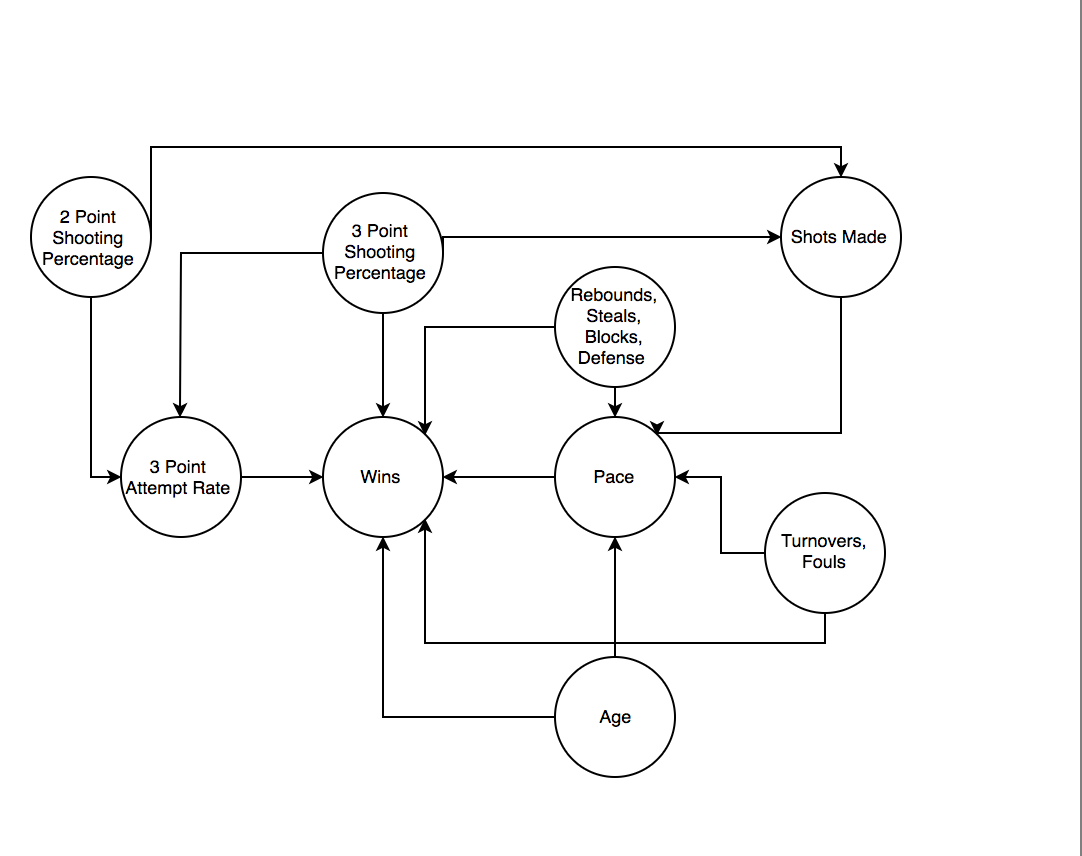
\includegraphics[width=0.5\textwidth, scale = 2]{causal}
\end{figure}
        	With regards to pace, anything that ends a possession and leads to wins would be a confounder. This includes rebounds, steals, blocks, fouls, turnovers, and making shots. Also, age is a major confounder for pace as older teams tend not to run as much push the pace as much.\par
        	As seen in our fixed effects model in model 3 below, everything is significant at the $\alpha$ = .01 level except for fouls, which is expected as all of these statistics should contribute to winning a basketball game. Age has a positive effect as once pace is controlled, as veterans are smarter and make better decisions than younger players. 3-point shooting percentage and 2-point shooting percentage both have positive effects on winning as expected along with rebounds, steals, and blocks. On the negative side, turnovers do have
a negative effect on winning a game.\par
\begin{table}[ht]
\def\tablename{Table}
\caption{Fixed Effects Model}
\centering
\begin{tabular}{lcccc}
\\
\hline \hline
& Estimates  &  Standardized Estimates  &  t-Ratio  &  p-value  \\
          
\hline

\\

3PAR  & 22.39  &       7.26 &                3.08 & .002            \\
Pace & 1.25 & .21 & -11.53 & p $<$ .0001\\
\\
Age & 4.97 & 0.434& 5.85 & p$<$.0001 \\
3PCT & 152.3 & 16.66 & 9.14 & p$<$.0001 \\
2PCT & 322.4 & 20.21 & 15.96 & p$<$.0001\\
TRB & .044 & .0024 & 18.2 & p$<$.0001\\
STL & .057 & .0047 & 12.19 & p$<$.0001\\
BLK & .015 & .0046 & 3.19& .0015\\
TOV& -.034 & .0038 & -9.24 & p$<$.0001\\
PF & -.00004 & .0028 & -.014 & .989\\

\\

\end{tabular}
\\ 
\scriptsize{$R^2 = .834$,  n = 30, T = 13,}\\

\end{table}


        	3-pointers attempted a game predicting wins has a very small p-value with a positive estimate. If this analysis is taken causally, it suggests that regardless of how the team shoots, a team should shoot more threes. Finally, pace had a negative estimate with a very small p-value, implying that given all the factors mentioned a faster game pace might not lead to better results. This result might suggest that teams should take fewer possessions in favor of longer, higher value possessions. \par
 
\section{Discussion and Conclusion}        	Using a fixed effects model and controlling for several possibly confounding factors, we conclude that regardless of a team's ability to shoot (within reason), a team should take more 3-pointers. This conclusion is in direct support of MoreyBall. However, our analysis also concluded that, when controlling for several turnover-causing factors, pace has a negative impact on winning. Although this appears contradictory to MoreyBall, it in fact is not entirely at odds. If a team is to play faster without any of the benefits of playing faster (better shots, more steals, etc.), then what is the point of playing fast? Our model controls for several of the benefits of playing fast. Thus, our causal graph might be incorrect in the fact that pace creates more opportunities for shots, steals, and blocks. There is a symbiotic relationship in that shots, steals, and blocks create more possessions and more possessions create more shots, steals, and blocks.  Unfortunately, like most things in statistics and basketball, it makes analyzing the effect of pace on a team much more difficult. We would conclude then that there's no evidence suggesting that a team should play fast if it can, but we would not refute pace as an important factor in the success of teams such as the Rockets and Warriors. \par
        	There are some adjustments to be made for this model to truly be predictive---although we referred to this analysis as predictive and causal during this paper, it would be more accurate to call these models descriptive. These models are more suited to knowing what lend themselves more to winning; actually predicting the outcomes of individual games will prove to be more difficult. We do have an idea of how to go about building a predictive model; however,  it would involve keeping comprehensive statistics
on every team (luckily, basketball-reference.com does this part for us) and fitting a model for each individual game. This approach could also be used to predict wins for a season before the season begins, involving lagged values and some measures for individual players (since every team is at least a little bit different at the beginning of each season). We believe a good way to predict success would be to
incorporate an instrumental variable for team chemistry. Although it would be hard to format, quantifying how many of the players have played together in other contexts (for example, Olympic teams, college teams, or All-Star teams) would be a fair instrument along with the number of mid-season head coaching fires a team has had.\par
        	Overall, this paper has suggests that MoreyBall is much more than just Morey
himself, and that his ideas, particularly shooting more 3-pointers, can be applied to any team. However, it would of course be more advantageous if the team taking more 3-pointers had some excellent 3-point shooters like James Harden as well.


\





\end{document}





